\documentclass[a4paper]{article}

%% Language and font encodings
\usepackage[utf8x]{inputenc}
\usepackage[italian]{babel}
\usepackage[T1]{fontenc}
\usepackage{multicol}
\usepackage{enumerate}
\usepackage[normalem]{ulem}
\usepackage{diagbox}
\usepackage{makecell}
\usepackage{booktabs}
\useunder{\uline}{\ul}{}
\usepackage{multirow}
\usepackage{tabularx}
\usepackage[bottom]{footmisc}
\usepackage{wrapfig}
\usepackage{graphicx}
\usepackage[table]{xcolor}
\usepackage{float}
\usepackage[font=small,labelfont=bf]{caption}
\usepackage{url}
\usepackage{subcaption}
\usepackage{chngcntr}
\usepackage{hyphenat}
\usepackage{amssymb}
\usepackage{amsmath}
\usepackage{cite}
\newcounter{rowno}
\counterwithin{figure}{section}
\counterwithin{table}{section}


\let\oldtexttt\texttt
\let\texttt\path


\definecolor{grigio_chiaro}{gray}{0.95}
\newcolumntype{h}{>{\columncolor{grigio_chiaro}}c}

%% Sets page size and margins
\usepackage[a4paper,
top=3cm,
bottom=3cm,
left=2cm,
right=2cm,
marginparwidth=1.75cm]{geometry}

%% Useful packages
\usepackage{amsmath}
\usepackage{graphicx}
\usepackage[colorinlistoftodos]{todonotes}
\usepackage[colorlinks=true, allcolors=blue]{hyperref}

\title{Analisi di Time Series, Sequential Pattern mining, \\  Classificazione e Outlier Detection \\ Data Mining 2, A.A. 2017/2018}


\author{Francesco Cariaggi \\ Leonardo Cariaggi \\ Luciana Latorraca}

\begin{document}

\maketitle
\tableofcontents

\newpage

\section{Introduzione}

In questa relazione riportiamo i risultati dei nostri esperimenti, effettuati utilizzando varie tecniche di Data Mining su differenti tipi di dati. Queste comprendono analisi e clustering di Time Series, Sequential Pattern mining mirato all'individuazione di pattern motfis-like, applicazione di vari modelli avanzati di classificazione e infine rilevamento degli \textit{outlier}. 

Nei due paragrafi immediatamente successivi illustreremo i due dataset su cui abbiamo concentrato i nostri studi, fornendo una panoramica dei dati.

\subsection{IBM stocks dataset}

Il dataset raggruppa in un'unica Time Series i valori delle azioni di IBM, azienda statunitense che opera nel settore informatico. I valori sono stati raccolti (più o meno) quotidianamente (con un totale di circa 250 valori invece di 365) in un arco di tempo di oltre 50 anni (dal 1962 al 2018). Utilizzeremo questo dataset esclusivamente nei primi due compiti (analisi di Time Series e mining di Sequential Pattern), raggruppando i dati per anno o per mese a seconda degli obiettivi.

\subsection{UCI Abalone dataset}

Questo dataset contiene delle misurazioni effettuate su 4177 abaloni, un genere di molluschi gasteropodi. La Tabella \ref{tab:semantics} descrive in maniera dettagliata le caratteristiche di ogni attributo degli abaloni.

\begin{table}[h]
\centering


\begingroup
\setlength{\tabcolsep}{8pt} % Default value: 6pt
\renewcommand{\arraystretch}{1.4} % Default value: 1
\rowcolors{1}{grigio_chiaro}{white}
\begin{tabularx}{\textwidth}{|llcX|}
\hline
\textbf{Nome dell'attributo} & \textbf{Tipo}                                                              & \textbf{Unità di misura} & \textbf{Descrizione}\\\hline

Sex & nominale & -- & Sesso dell'abalone. Può assumere i valori M, F o I (infante). \\

Length & continuo & mm & Misura della conchiglia più lunga. \\
Diameter & continuo & mm & Diametro della conchiglia, misurato perpendicolarmente alla lunghezza. \\
Height & continuo & mm & Altezza misurata con il mollusco dentro la conchiglia. \\
Whole weight & continuo & g & Peso dell'intero abalone. \\
Shucked weight & continuo & g & Peso del solo mollusco. \\
Viscera weight & continuo & g & Peso delle interiora del mollusco. \\
Shell weight & continuo & g & Peso della sola conchiglia (dopo l'asciugatura). \\
Rings & intero & -- & Numero di anelli nella conchiglia. Se lo sommiamo a 1.5, otteniamo l'età in anni dell'abalone. \\

 \hline
\end{tabularx}
\endgroup
\caption{Semantica dei dati}
\label{tab:semantics}
\end{table}



\newpage

\section{Time series}


In questa sezione si discute lo studio delle similarità e l'analisi dei cluster tra Time Series. Quelle utilizzate negli esperimenti sono state ottenute suddividendo quella originale in 57 serie annuali e normalizzando i valori utilizzando la normalizzazione \textit{Z-score}. L'obiettivo che ci prefissiamo in questo contesto è riuscire ad individuare i particolari che accomunano certi gruppi di Time Series e darne una chiave di lettura.

\subsection{Autocorrelazione}

L'autocorrelazione è una misura del grado di dipendenza tra i valori di una Time Series e una copia traslata nel tempo di essa stessa. Un valore prossimo allo zero indica che i valori della serie hanno una distribuzione pressoché casuale. Si usa l'autocorrelazione principalmente per individuare porzioni di Time Series che si ripetono periodicamente: in tal caso, si parla di autocorrelazione positiva. La Figura \ref{fig:autocorr_plot} illustra il grado di autocorrelazione di tutte le 57 Time Series annuali.

\begin{figure}[h]
	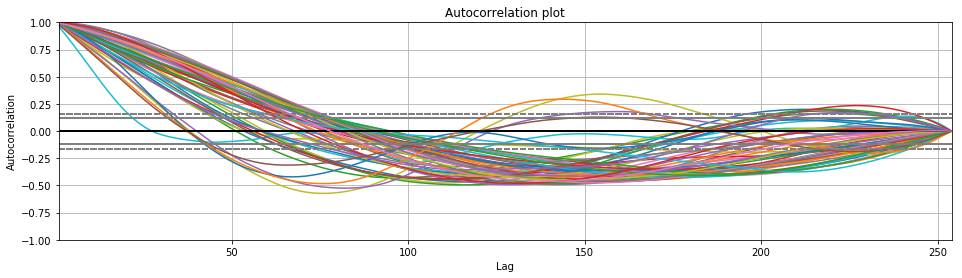
\includegraphics[width=\textwidth]{images/autocorrelation_plot.png}
	\caption{Grafico di autocorrelazione delle Time Series}
	\label{fig:autocorr_plot}
\end{figure}

\noindent
Se non consideriamo gli alti livelli di correlazione nella parte iniziale del grafico, dovuti a valori troppo bassi del \textit{lag}, notiamo che dalla figura emerge il fenomeno opposto a quello descritto all'inizio del paragrafo: intorno a metà anno (indicativamente verso il mese di Giugno), infatti, il livello di autocorrelazione di quasi tutte le serie eccede negativamente la soglia, arrivando a circa $-0.5$. Ciò suggerisce che il valore delle azioni nel sesto mese del calendario segue un andamento tendenzialmente opposto rispetto a quello di inizio anno (perfettamente opposto se il grado di correlazione fosse stato $-1$).



\subsection{Stazionarietà}

La non stazionarietà di una Time Series è indice del fatto che essa ha una struttura dipendente dal tempo. In altre parole, la serie è affetta da fenomeni che portano alcuni parametri (per esempio media, varianza ecc.) a cambiare nel tempo, come ad esempio la presenza di trend o di stagionalità. L'\textit{Augmented Dickey-Fuller unit root test} fornisce una buona stima della stazionarietà di una Time Series. La Figura \ref{fig:dickey_fuller} è il risultato dell'applicazione del suddetto test alle serie annuali.

\begin{figure}[h]
	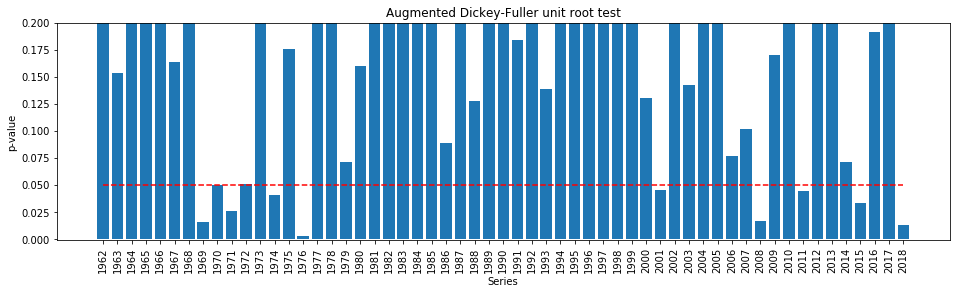
\includegraphics[width=\textwidth]{images/dickey_fuller.png}
	\caption{Augmented Dickey-Fuller unit root test}
	\label{fig:dickey_fuller}
\end{figure}

Per determinare la stazionarietà di una serie occorre fare riferimento al \textit{p-value}: se questo è minore di $0.05$, allora diciamo che la serie è stazionaria. Altrimenti, si trae la conclusione opposta. Dalla Figura \ref{fig:dickey_fuller} emerge che la quasi totalità delle serie possiede un \textit{p-value} ben al di sopra del valore critico (il grafico è stato tagliato a $0.2$ solo per questioni di leggibilità): ciò rivela la presenza di stagionalità all'interno delle Time Series.

\subsection{Clustering}

Uno degli obiettivi che ci siamo prefissati è quello di individuare gruppi di Time Series che condividono simili caratteristiche. In questo paragrafo sperimenteremo alcuni algortmi di clustering e confronteremo i risultati ottenuti.

\subsubsection{Clustering con DBSCAN}

Il primo algoritmo di clustering che abbiamo sperimentato è DBSCAN (\textit{Density-Based Spatial Clustering of Applications with Noise}). Esso è particolarmente adatto in situazioni in cui i cluster non possiedono una forma sferica e la loro densità è sufficientemente omogenea.

I parametri da fornire sono due: il primo, $min\_pts$, definisce il numero minimo di vicini di un punto per considerarlo un \textit{core point} \cite{dbscan}; il secondo, $\epsilon$, definisce invece la distanza entro la quale cercare tali vicini. Per il calcolo della matrice della distanze tra le Time Series abbiamo considerato due opzioni: la distanza Euclidea e la \textit{Dynamic Time Warping} (DTW). Sebbene non ci sia una differenza rilevante, nel primo caso (Figura \ref{subfig:eucl}) le distanze sono leggermente più alte. Per questo motivo abbiamo optato per la seconda opzione (Figura \ref{subfig:dtw}).

\begin{figure}[h]
\centering
\begin{subfigure}[b]{.30\linewidth}
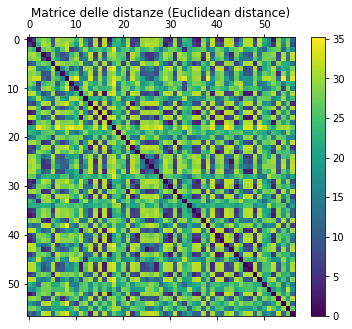
\includegraphics[width=\linewidth]{images/euclidean.png}
\caption{Distanza Euclidea}
\label{subfig:eucl}
\end{subfigure}
\begin{subfigure}[b]{.30\linewidth}
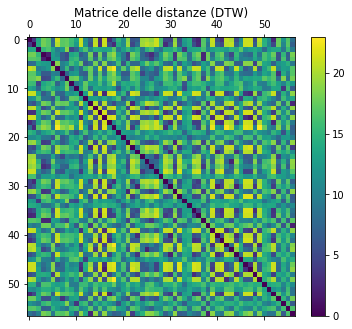
\includegraphics[width=\linewidth]{images/dtw_sqrt.png}
\caption{DTW}
\label{subfig:dtw}
\end{subfigure}
\caption{Matrici delle distanze tra le Time Series}
\label{fig:distance_matrixes}
\end{figure}

La Figura \ref{fig:choice_minpts} mostra la modalità di scelta del parametro $min\_pts$: la nostra strategia consiste nel disegnare i valori ordinati delle distanze dei punti dai propri $k$ vicini più prossimi (nel nostro caso abbiamo provato valori per $k \in \{2,4,6,8,10,12\}$) e poi prendere il punto di "gomito". In ognuna delle alternative, otteniamo un punto di "gomito" in $min\_pts=3$.

\begin{figure}[h]
	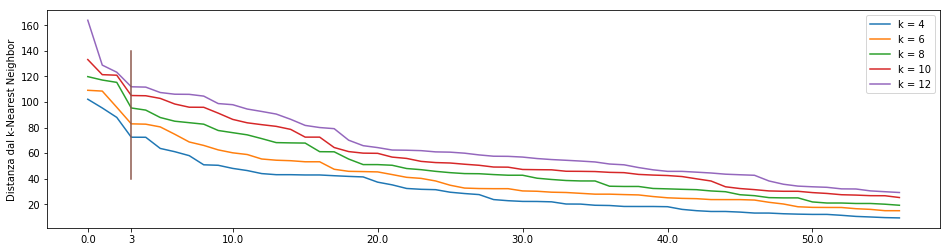
\includegraphics[width=\textwidth]{images/choice_of_minpts.png}
	\caption{Scelta del parametro $min\_pts$ per l'algoritmo DBSCAN}
	\label{fig:choice_minpts}
\end{figure}

Riguardo il parametro $\epsilon$, invece, abbiamo provato eseguito l'algoritmo per tutti i valori compresi nell'intervallo $[70,120]$ (sempre in accordo alla Figura \ref{fig:choice_minpts}, ma stavolta in riferimento all'asse delle ordinate). Poi, per ogni esecuzione, abbiamo registrato il valore della \textit{silhouette}, riportando tutto in Figura \ref{fig:silhouette_vs_epsilon}.

\begin{figure}[h]
	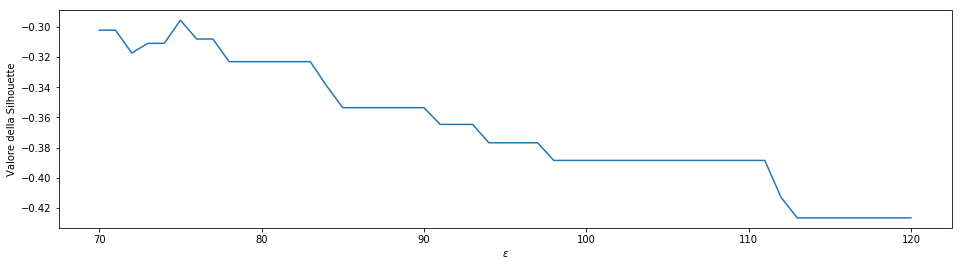
\includegraphics[width=\textwidth]{images/silhouette_vs_epsilon.png}
	\caption{Valore della \textit{silhouette} per diversi valori del parametro $\epsilon$ per l'algoritmo DBSCAN}
	\label{fig:silhouette_vs_epsilon}
\end{figure}

Come testimoniato dai risultati ottenuti, tuttavia, DBSCAN esibisce un comportamento piuttosto deludente. Il valore della \textit{silhouette} è sempre negativo, ad indicare che le Time Series non sono state assegnate ai cluster appropriati.

\subsubsection{Clustering con K-means}

Per il clustering delle Time Series abbiamo sperimentato anche l'algoritmo K-means, utilizzando la distanza Euclidea  come metrica di comparazione. Per rilevare i cluster, questo algoritmo punta a minimizzare l'\textit{SSE} (Sum of Squared Error), che è una misura della distanza di ogni elemento dal centroide del rispettivo cluster. Non sempre un basso SSE è sinonimo di buon risultato: se decidessimo infatti di definire un cluster per ogni singolo punto, l'SSE sarebbe uguale a zero, ma ovviamente il risultato sarebbe scarso dal punto di vista informativo. L'obiettivo cruciale è quindi riuscire a trovare un compromesso tra SSE e numero di cluster. La Figura \ref{fig:SSE_curve} mostra una valida strategia (punto di "gomito") per la scelta ottimale del numero di cluster.

\begin{figure}[h]
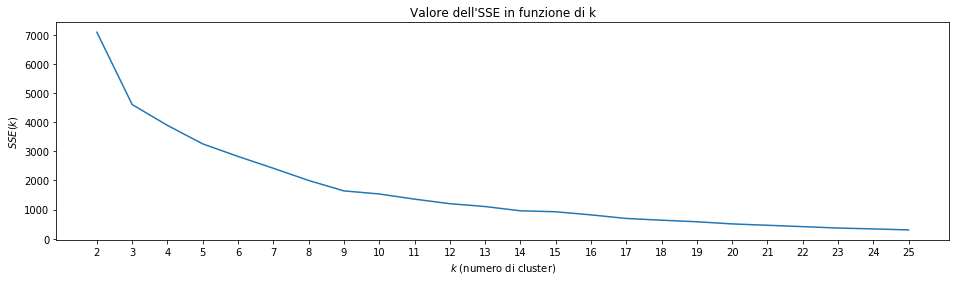
\includegraphics[width=\textwidth]{images/SSE_curve.png}
\caption{Andamento dell'SSE all'aumentare del numero di cluster. $k=3$ è il punto di gomito}
\label{fig:SSE_curve}
\end{figure}

Per $k=3$ notiamo che l'SSE subisce una diminuzione significativa, perciò ragionevolmente la nostra scelta del numero di cluster ricade sul numero $3$. Per valori di $k$ maggiori di 3, la pendenza della curva non è abbastanza accentuata da giustificare la scelta di un numero di cluster in quell'intervallo.
Fissando dunque il parametro nel modo sopra descritto, l'esecuzione dell'algoritmo rivela la presenza di tre cluster ben definiti. 

Nella Figura \ref{fig:cluster_visualization} possiamo distinguere chiaramente le caratteristiche delle Time Series in ognuno dei cluster. In particolare, nel primo cluster troviamo le serie che corrispondono ad un andamento crescente del valore delle azioni. Qui sono dunque raggruppati quelli che potremmo definire i tempi d'oro dell'azienda, ovvero gli anni in cui essa ha goduto di una forte crescita.

Il secondo cluster, invece, evidenzia una situazione opposta rispetto a quella del primo: queste serie infatti testimoniamo un preoccupante calo delle azioni, come a suggerire che in quegli anni l'azienda fosse stata travolta da una grave crisi di mercato.

Nel terzo cluster, le Time Series riflettono invece un comportamento altalenante, caratterizzato dapprima da una diminuzione e in seguito da un aumento: intuitivamente, il valore di mercato delle azioni negli anni corrispondenti a quelle serie è lo stesso sia a inizio che a fine anno, con un calo significativo nei mesi centrali.

\begin{figure}[h]
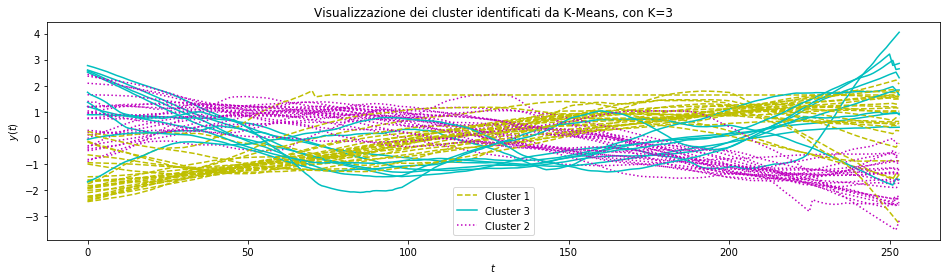
\includegraphics[width=\textwidth]{images/cluster_visualization.png}
\caption{Visualizzazione dei cluster individuati da K-means, con $k=3$}
\label{fig:cluster_visualization}
\end{figure}

A ulteriore conferma dei nostri risultati, la Figura \ref{fig:cluster_heatmap} presenta lo stesso concetto sottoforma di \textit{Heatmap}: ad un colore blu corrispondono valori bassi delle azioni, mentre ad un colore verde/giallo corrispondono valori alti. Leggendo il grafico dall'alto verso il basso, possiamo distinguere nell'ordine il primo, il secondo e il terzo cluster. Un aspetto che non viene ben evidenziato dalla figura precedente (Figura \ref{fig:cluster_visualization}), ma che invece è ben rappresentato dall'\textit{Heatmap}, è la quantità di serie in ogni cluster: sembra infatti che nei primi due cluster la quantità di serie sia pressoché identica, mentre nel terzo è decisamente minore.

\begin{figure}[h]
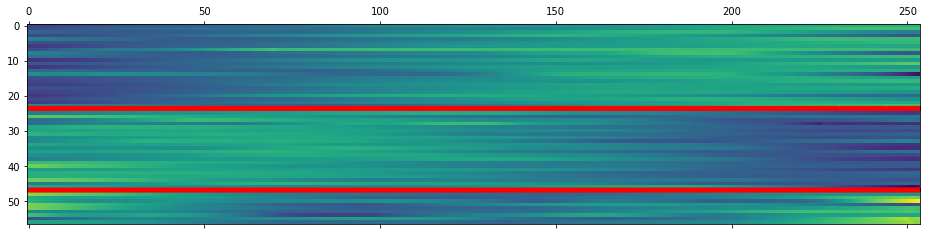
\includegraphics[width=\textwidth]{images/matshow_clusters.png}
\caption{Visualizzazione dei cluster individuati da K-means tramite \textit{Heatmap}}
\label{fig:cluster_heatmap}
\end{figure}

\subsubsection{Clustering tramite feature-extraction}

Come ultima alternativa abbiamo anche preso in considerazione l'utilizzo di tecniche basate su \textit{feature-extraction}. Nello specifico, abbiamo sperimentato una \textit{feature-extraction} basata sulla trasformata di Fourier applicata a K-means \cite{introtodm}. In questo caso la qualità dei risultati è nettamente inferiore a quella dei precedenti algoritmi. In Figura \ref{fig:fourier_cluster} si vede chiaramente che l'algoritmo non riesce a definire i cluster in maniera chiara.

\begin{figure}[h]
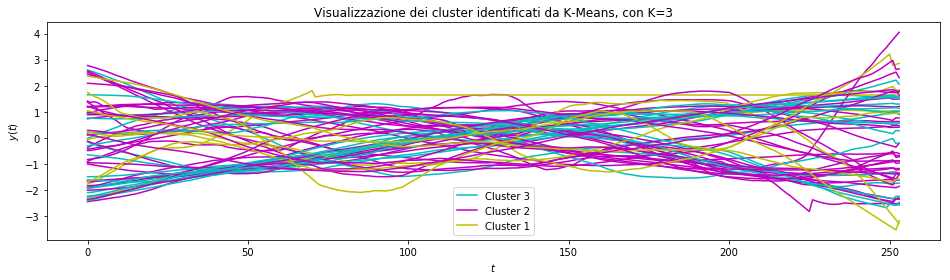
\includegraphics[width=\textwidth]{images/fourier_clusters.png}
\caption{Visualizzazione dei cluster individuati da K-means, con \textit{feature extraction} basata sulla trasformata di Fourier}
\label{fig:fourier_cluster}
\end{figure}

\subsection{Conclusioni}

Dall'analisi delle Time Series annuali abbiamo potuto individuare la presenza di particolari fenomeni, come l'autocorrelazione e la non stazionarietà. Attraverso il clustering con K-means si è potuto osservare quali fossero le caratteristiche comuni a più serie, cercando di interpretare da un punto di vista "economico" i risultati ottenuti. Per motivi riguardanti la distribuzione dei cluster e la lunghezza delle serie, nessuna delle altre tecniche di clustering è riuscita ad ottenere risultati significativi.

\newpage

\section{Sequential Patterns}

Gli esperimenti di questa sezione riguardano lo stesso dataset utilizzato nella sezione precedente. L'obiettivo è l'individuazione di \textit{Sequential Pattern} nelle Time Series dei valori delle azioni dell'azienda \textit{IBM}. In questo contesto, tuttavia, le serie all'interno delle quali cercare i pattern sono state ottenute suddividendo quella originale in 676 serie mensili. 

A questo scopo abbiamo effettuato una normalizzazione \textit{Z-score} e una discretizzazione dei valori delle serie, utilizzando dei bin ad ampiezza costante. In conseguenza a questa scelta abbiamo ritenuto opportuno rimuovere il \textit{trend} lineare presente nella Time Series originale, usando l'\textit{exponential decay}. Nei paragrafi successivi illustreremo le differenze tra i risultati ottenuti scegliendo di discretizzare i dati (\textit{i}) prima della suddivisione in serie mensili (che indicheremo con \textit{discretizzazione anticipata}) e (\textit{ii}) dopo la suddivisione (\textit{discretizzazione posticipata}).

Riguardo al rumore presente nella serie, abbiamo deciso di effettuare esperimenti sia in sua presenza che in sua assenza (rimuovendolo sostituendo i valori della serie con il valore medio dei propri vicini).

Per individuare i pattern abbiamo utilizzato l'algoritmo GSP esteso con i vincoli temporali (\textit{Generalized Sequential Pattern Mining with Item Intervals}, \cite{hirate}). Le specifiche richiedevano di trovare sottosequenze contigue di lunghezza $\geq$ 4, dunque è stato sufficiente impostare $max\_gap = 1$ e $min\_span = 3$.

\subsection{Sequential Patterns con discretizzazione posticipata}

In questa variante si è deciso processare i dati seguendo questo ordine:

\begin{enumerate}
	\item Suddivisione della Time Series originale in 676 serie mensili;
	\item Normalizzazione \textit{Z-score} dei valori in ciascuna serie ottenuta;
	\item Discretizzazione dei valori, utilizzando 8 bin di ampiezza fissa.
\end{enumerate}

Dal momento che ognuna delle serie mensili consiste di circa 20/25 elementi, abbiamo ritenuto ragionevole l'utilizzo di un numero di bin non troppo alto e, allo stesso tempo, che fosse sufficientemente adatto a rappresentare in maniera dettagliata la varietà dei valori delle serie.

\begin{table}[h]
\centering
\begingroup
\setlength{\tabcolsep}{5pt} % Default value: 6pt
\renewcommand{\arraystretch}{1.8} % Default value: 1
%\rowcolors{1}{grigio_chiaro}{white}
\begin{tabularx}{0.7\textwidth}{|h|X|X|X|X|}
\hline
\rowcolor{grigio_chiaro}
\diagbox{Configurazione}{$min\_sup$}& \textbf{0.1} & \textbf{0.2} & \textbf{0.3} & \textbf{0.4} \\ \hline
Num. pattern (serie con noise) & 11 & 0 & 0 & 0 \\ \hline
Num. pattern (serie senza noise) & 260 & 78 & 23 & 11 \\ \hline
\end{tabularx}
\endgroup
\caption{Numero di \textit{Sequential Pattern} trovati per diverse configurazioni}
\label{tab:number_of_patterns}
\end{table}

La Tabella \ref{tab:number_of_patterns} riassume i risultati dei nostri esperimenti. Prima di tutto osserviamo che lo stesso tipo di esperimenti è stato replicato due volte, considerando sia (\textit{i}) la Time Series originale (non privata del rumore) che (\textit{ii}) la Time Series privata del rumore. La cosa interessante da notare è che, nel primo caso, gli unici pattern frequenti sono quelli aventi un supporto di circa il $10\%$ (11 in totale). Nessun pattern è stato trovato per valori maggiori del supporto. Ciò è principalmente causato dalla presenza del rumore, che comporta inevitabilmente un'elevata variabilità dei dati.

Nel secondo caso, invece, osserviamo che con il medesimo valore di $min\_sup$ (cioè il $10\%$) otteniamo ben 260 pattern frequenti. Inoltre, all'aumentare della soglia minima del supporto, il numero di pattern rimane sempre sopra lo zero. In particolare, ci sono 11 pattern aventi un supporto non inferiore al $40\%$.


\begin{table}[h]
\centering
\begingroup
\setlength{\tabcolsep}{5pt} % Default value: 6pt
\renewcommand{\arraystretch}{1.8} % Default value: 1
%\rowcolors{1}{grigio_chiaro}{white}
\begin{tabularx}{\textwidth}{|X|X|X|X|X|}
\hline
\rowcolor{grigio_chiaro}
\diagbox[font=\footnotesize\itshape]{Config.}{$min\_sup$}& \textbf{0.1} & \textbf{0.2} & \textbf{0.3} & \textbf{0.4} \\ \hline

Esempi \newline (noise)
& [ $6,7,7,7$ ] 
	\par [ $0,0,0,1$ ] 
	\newline [ $7,6,6,5$ ] 
& $\emptyset$
& $\emptyset$ 
& $\emptyset$ \\ \hline

Esempi \newline (no noise)
& [$3,3,4,4,5,5,6,6,6$] 
	\newline [$2,2,3,3,4,4,5,5$] 
	\newline [$4,3,3,2,2,1,1$] 
& [$2,3,3,4$] 
	\newline [$5,6,6,7$] 
	\newline [$3,2,2,1$] 
& [$1,1,0,0,0$] 
	\newline [$3,4,4,5$] 
	\newline [$7,7,7,7$] 
& [$5,5,6,6$] 
	\newline [$0,0,1,1$] 
	\newline [$6,7,7,7$] 
\\\hline

\end{tabularx}
\endgroup
\caption{Alcuni esempi di \textit{Sequential Pattern} per diverse configurazioni}
\label{tab:example_patterns}
\end{table}

Nella Tabella \ref{tab:example_patterns} sono riportati alcuni esempi di pattern frequenti. Dal momento che abbiamo discretizzato utilizzando 8 bin, i pattern sono rappresentati con valori (da 0 a 7) che indicano a quale bin appartiene il valore originale. Osserviamo che il pattern [6,7,7,7] ha una frequenza ben diversa nei due casi: nel primo si aggira intorno al $10\%$, mentre nel secondo caso supera il $40\%$. In più possiamo confermare che in assenza di rumore nei dati i pattern sono tipicamente più estesi (più lunghi di 4 giorni).

Un'altro aspetto interessante rivelato dalla Tabella \ref{tab:example_patterns} è il fatto che i pattern frequenti contengono sempre valori consecutivi che differiscano al massimo di un'unità (un bin). Si deduce quindi che, all'interno delle Time Series, è improbabile che si verifichino dei bruschi cambiamenti.

Infine, la Figura \ref{fig:patterns} ci permette di visualizzare graficamente alcuni dei pattern frequenti rilevati in precedenza. Nella Figura \ref{subfig:pat_noise} sono riportate le occorrenze del pattern [7,7,6,5], che compare principalmente nelle serie caratterizzate da un'evidente andamento discendente. Intuitivamente, questi sono i mesi nei quali le azione dell'azienda hanno subito un calo.

La Figura \ref{subfig:pat_no_noise} mostra invece il pattern [3,3,4,4,5,5,6,6,6]: le serie che lo contengono hanno sostanzialmente la stessa struttura, che suggerisce un incremento costante del valore delle azioni.

\begin{figure}[h]
\centering
\begin{subfigure}[b]{\linewidth}
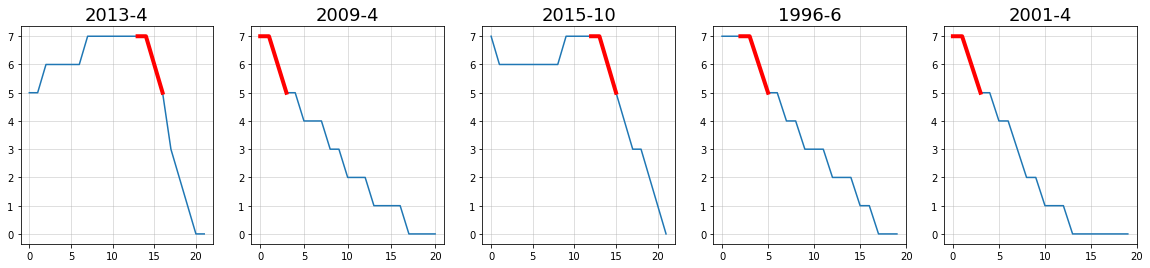
\includegraphics[width=\linewidth]{images/discr_poi_noise.png}
\caption{Visualizzazione del pattern [7,7,6,5] (Time Series con noise)}
\label{subfig:pat_noise}
\end{subfigure}
\begin{subfigure}[b]{\linewidth}
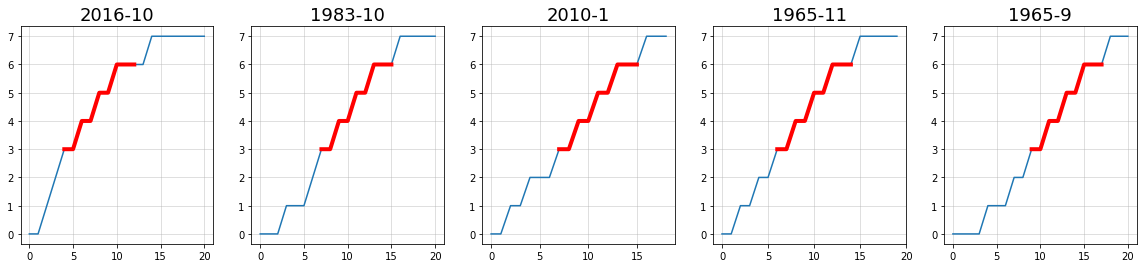
\includegraphics[width=\linewidth]{images/discr_poi_no_noise.png}
\caption{Visualizzazione del pattern [3,3,4,4,5,5,6,6,6] (Time Series senza noise)}
\label{subfig:pat_no_noise}
\end{subfigure}
\caption{Visualizzazione di alcuni dei pattern frequenti nelle corrispondenti Time Series mensili}
\label{fig:patterns}
\end{figure}

\subsection{Conclusioni}
In questa sezione abbiamo condotto diversi esperimenti sulle Time Series mensili, con l'obiettivo di trovare al loro interno dei pattern frequenti. Abbiamo potuto constatare le conseguenze derivanti dalla rimozione del rumore dalla serie originale, mettendo in risalto le principali differenze rispetto all'analisi dei dati grezzi. Abbiamo inoltre osservato l'importanza della discretizzazione che, a seconda del momento in cui viene effettuata, porta a risultati completamente differenti.


\newpage

\section{Classificazione}

Nelle sezioni che seguono sono riportati i risultati ottenuti da vari modelli di classificazione sul dataset \emph{Abalone}\footnote{https://archive.ics.uci.edu/ml/datasets/Abalone}.

\subsection{Preprocessamento del dataset}
Si è inizialmente proceduto a rimuovere gli abaloni "bambini" (ossia quelli aventi $Sex=I$), lasciando solamente maschi ($Sex=M$) e femmine ($Sex=F$). L'attributo $Sex$ è stato inoltre convertito in valori numerici per ragioni di compatibilità con le librerie utilizzate.

Si è scelto inoltre di rimuovere l'attributo $Diameter$ in quanto fortemente correlato (con un indice di circa 0.97 secondo la metrica di Pearson) con l'attributo $Length$. La Figura \ref{fig:corr}, infatti, dimostra che esiste una significativa correlazione lineare fra i due attributi.

L'attributo $Rings$ è stato discretizzato usando due intervalli, ricavati osservando la distribuzione dell'attributo. La Figura \ref{fig:KDE_Rings} evidenzia che l'attributo presenta una distribuzione simile ad una $\mathcal{N}(10, \sigma^2)$. Per tale motivo, si è deciso di discretizzare $Rings$ in due classi secondo la regola:
\begin{itemize}
	\item $Rings<10 \implies$ classe $0$
	\item $Rings \geq 10 \implies$ classe $1$	
\end{itemize}


%\begin{figure}[h]
%\centering
%\begin{minipage}{.45\textwidth}
%	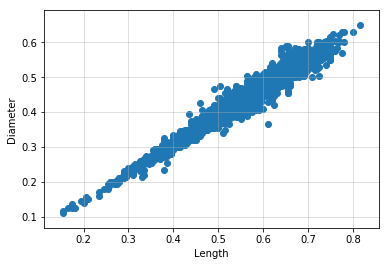
\includegraphics[width=\textwidth]{images/corr.png}
%	\caption{"Length" e "Diameter" a confronto}
%	\label{fig:corr}
%\end{minipage}\hfill
%\begin{minipage}{.45\textwidth}
%	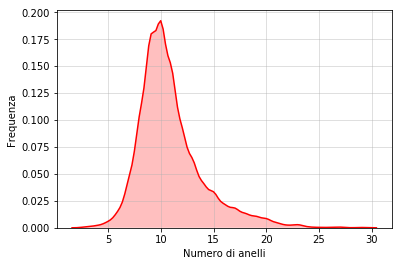
\includegraphics[width=\textwidth]{images/kde_rings.png}
%	\caption{Distribuzione dell'attributo "Rings"}		
%\label{fig:KDE_Rings}
%\end{minipage}
%\end{figure}


\begin{figure}[h]
\centering
\begin{subfigure}[b]{.48\linewidth}
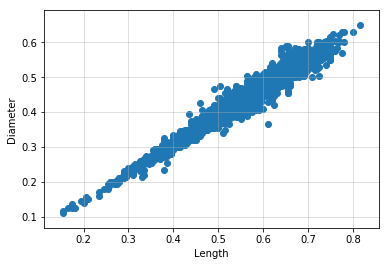
\includegraphics[width=\linewidth]{images/corr.png}
\caption{"Length" e "Diameter" a confronto}
	\label{fig:corr}
\end{subfigure}
\begin{subfigure}[b]{.48\linewidth}
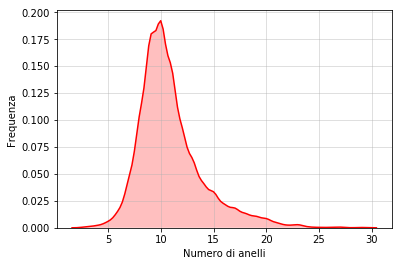
\includegraphics[width=\linewidth]{images/kde_rings.png}
\caption{Distribuzione dell'attributo "Rings"}	
\label{fig:KDE_Rings}
\end{subfigure}
\caption{Statistiche su alcuni attributi del dataset}
\label{fig:abalone_stats}
\end{figure}

\subsection{Classificazione con Naïve-Bayes}

In questa sezione sono riportati i risultati ottenuti impiegando un modello Naïve Bayes gaussiano. Il modello è stato valutato mediante un processo di cross-validation con 20 fold. Le metriche utilizzate sono state accuratezza e AUC (area sottesa dalla curva ROC del modello). La Figura \ref{fig:naivebayes} riporta i valori di tali misure in ciascuna delle 20 fold della cross-validation. \`{E} possibile notare come l'accuratezza e il valore della AUC rimangano pressoché stabili negli insiemi di training (intorno al 65\% e al 70\%, rispettivamente), mentre si ha una vistosa fluttuazione nei vari insiemi di test. In alcune fold, ad esempio, il modello sembra funzionare molto bene (accuratezza oltre l'80\% e AUC che sfiora il 100\%), mentre in altre ha prestazioni perfino inferiori al modello random (accuratezza ed AUC intorno al 30\%).

\begin{figure}[h]
	\centering
	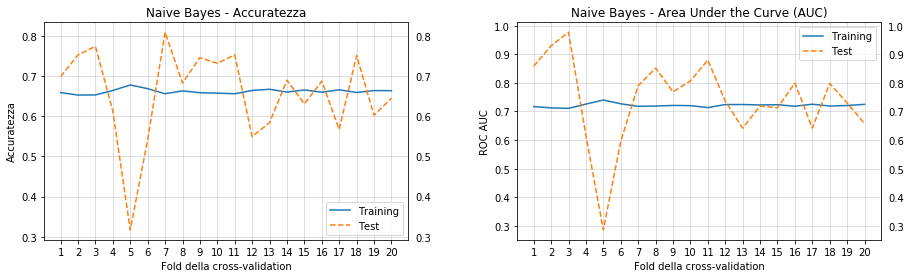
\includegraphics[width=\textwidth]{images/naivebayes.png}
	\caption{Risultati ottenuti con un modello Naive Bayes}		
\end{figure}
\label{fig:naivebayes}


\subsection{Classificazione con SVM}
La valutazione delle performance del modello è avvenuta per mezzo di una grid search esaustiva, esplorando un ampio spettro di possibili iperparametri. Per ogni iperparametro sono stati testati i seguenti valori:
\begin{itemize}
\item \textbf{Kernel}
	\begin{itemize}
	\item[$\rightarrow$] Lineare: $\phi(x, y) = x^Ty$
	\item[$\rightarrow$] Polinomiale: $\phi(x, y) = (\gamma \cdot x^Ty + r)^d$
	\item[$\rightarrow$] Gaussiano (o RBF): $\phi(x, y) = e^{-\gamma \cdot||x-y||^2}$
	\item[$\rightarrow$] Sigmoideo: $\phi(x, y) = tanh(\gamma \cdot x^Ty + r)$
	\end{itemize}
\item \textbf{C} (fattore di penalizzazione delle \emph{slack variables} $\xi_i$) $\rightarrow$ $1$, $10$, $10^2$, $10^3$
\item $\pmb{\gamma}$ (solo per kernel polinomiale, gaussiano o sigmoideo) $\rightarrow$ $10^{-4}$, $10^{-3}$, $10^{-2}$, $10^{-1}$
\item $\mathbf{d}$ (grado del polinomio, solo per kernel polinomiale) $\rightarrow$ 2, 3, 4, 5, 6, 7, 8, 9, 10
\item $\mathbf{r}$ (termine noto, solo per kernel polinomiale e sigmoideo) $\rightarrow$ -1, 0, 1
\end{itemize}
\noindent
Per ciascuna combinazione di tali iperparametri, inoltre, è stata effettuata una cross validation con 3 fold.

La Tabella \ref{tab:svm} riporta i risultati dei 5 migliori modelli testati, ordinati in maniera decrescente secondo l'accuratezza ottenuta negli insiemi di test. Tale valore si riferisce alla media dei valori ottenuti in ciascuna delle diverse fold della cross validation, accanto alla quale si riporta anche il doppio della deviazione standard. In caso di parità, vengono valutati, in ordine, le misure di: AUC media negli insiemi di test, deviazione standard dell'accuratezza negli insiemi di test, deviazione standard dell'AUC negli insiemi di test.

Il valore dell'accuratezza del modello vincente è riportato in grassetto. Si può notare, comunque, che i 5 modelli hanno prestazioni molto simili. Lo stesso si può dire degli iperparametri.

\begin{table}[h]
\centering
\begingroup
\setlength{\tabcolsep}{5pt} % Default value: 6pt
\renewcommand{\arraystretch}{1.8} % Default value: 1
%\rowcolors{1}{grigio_chiaro}{white}
\begin{tabularx}{\textwidth}{|h|X|X|X|X|X|}
\hline
\rowcolor{grigio_chiaro}
& \textbf{Modello 1} & \textbf{Modello 2} & \textbf{Modello 3} & \textbf{Modello 4} & \textbf{Modello 5} \\ \hline
Kernel & Polinomiale & Gaussiano & Polinomiale & Polinomiale & Polinomiale \\ \hline
$C$ & $10^{3}$ & $10^{3}$ & $10^{3}$ & $10^{3}$ & $10^{2}$ \\ \hline
$\gamma$ & $10^{-2}$ & $10^{-1}$ & $10^{-1}$ & $10^{-1}$ & $10^{-1}$ \\ \hline
$d$ & 10 & - & 3 & 2 & 5 \\ \hline
$r$ & 1 & - & 1 & 1 & 1 \\ \hline
Accuratezza media (Training) & $0.768 \pm 0.024$ & $0.772 \pm 0.026$ & $0.770 \pm 0.024$ & $0.769 \pm 0.022$ & $0.769 \pm 0.024$ \\ \hline
Accuratezza media (Test) & $\mathbf{0.769} \pm 0.045$ & $0.768 \pm 0.049$ & $0.768 \pm 0.050$ & $0.767 \pm 0.045$ & $0.766 \pm 0.046$ \\ \hline
AUC media (Training) & $0.829 \pm 0.022$ & $0.830 \pm 0.020$ & $0.831 \pm 0.020$ & $0.830 \pm 0.022$ & $0.830 \pm 0.020$ \\ \hline
AUC media (Test) & $0.820 \pm 0.047$ & $0.819 \pm 0.045$ & $0.819 \pm 0.046$ & $0.821 \pm 0.045$ & $0.818 \pm 0.046$ \\ \hline
\end{tabularx}
\endgroup
\caption{Risultati ottenuti con una SVM}
\label{tab:svm}
\end{table}

\subsection{Classificazione con Rete Neurale}

Per allenare la rete neurale si è scelto di impiegare il metodo della discesa del gradiente, adottando anche alcune delle più comuni euristiche quali momento di Nesterov e regolarizzazione di Tikhonov \cite{dlbook}.

Poiché una ricerca esaustiva avrebbe richiesto uno sforzo computazionale eccessivo, si è scelto di procedere come in \cite{randsearch}, scegliendo ogni volta in maniera casuale una certa configurazione di iperparametri. Nel nostro caso, si è scelto di testare 500 configurazioni casuali. Di seguito sono riportati i valori possibili per ciascun iperparametro:

\begin{itemize}
\item \textbf{Unità nascoste} $\rightarrow$ $\{(h, -)\,\, | \,\,h \in [3, 10]\,\} \cup \{(h_1, h_2)\,\, | \,\,h_1, h_2 \in [3, 10]\}$, dove $(h, -)$ denota $h$ unità nell'unico livello nascosto, e $(h_1, h_2)$ denota $h_1$ unità nel primo livello nascosto ed $h_2$ unità nel secondo livello nascosto
\item \textbf{Learning rate} $\rightarrow$ $10^{-4}$, $10^{-3}$, $10^{-2}$, $10^{-1}$
\item \textbf{Momento} $\rightarrow$ 0.3, 0.4, 0.5, 0.6, 0.7, 0.8, 0.9
\item \textbf{Fattore di regolarizzazione di Tikhonov} $\rightarrow$ $10^{-6}$, $10^{-5}$, $10^{-4}$, $10^{-3}$, $10^{-2}$
\end{itemize}

La Tabella \ref{tab:neural_network} riporta i risultati ottenuti dalla rete neurale, che sono leggermente peggiori di quelli della SVM. Anche in questo caso, le prestazioni dei diversi modelli non presentano differenze significative.

\begin{table}[h]
\centering
\begingroup
\setlength{\tabcolsep}{5pt} % Default value: 6pt
\renewcommand{\arraystretch}{1.8} % Default value: 1
%\rowcolors{1}{grigio_chiaro}{white}
\begin{tabularx}{\textwidth}{|h|X|X|X|X|X|}
\hline
\rowcolor{grigio_chiaro}
& \textbf{Modello 1} & \textbf{Modello 2} & \textbf{Modello 3} & \textbf{Modello 4} & \textbf{Modello 5} \\ \hline
Livelli nascosti & 2 & 2 & 2 & 2 & 2 \\ \hline
Unità nascoste & (4, 10) & (8,10) & (9, 7) & (8, 6) & (4, 8) \\ \hline
Learning rate & $10^{-2}$ & $10^{-2}$ & $10^{-2}$ & $10^{-2}$ & $10^{-2}$ \\ \hline
Momento & 0.9 & 0.9 & 0.9 & 0.9 & 0.9 \\ \hline
Regolarizzazione & $10^{-2}$ & $10^{-4}$ & $10^{-4}$ & $10^{-6}$ & $10^{-4}$ \\ \hline
Accuratezza media (Training) & $0.753 \pm 0.022$ & $0.752 \pm 0.028$ & $0.752 \pm 0.024$ & $0.751 \pm 0.026$ & $0.748 \pm 0.020$ \\ \hline
Accuratezza media (Test) & $\mathbf{0.749} \pm 0.026$ & $0.745 \pm 0.032$ & $0.745 \pm 0.040$ & $0.745 \pm 0.036$ & $0.745 \pm 0.036$ \\ \hline
AUC media (Training) & $0.810 \pm 0.034$ & $0.811 \pm 0.026$ & $0.813 \pm 0.020$ & $0.811 \pm 0.028$ & $0.809 \pm 0.028$ \\ \hline
AUC media (Test) & $0.807 \pm 0.040$ & $0.808 \pm 0.052$ & $0.808 \pm 0.058$ & $0.804 \pm 0.052$ & $0.803 \pm 0.050$ \\ \hline
\end{tabularx}
\endgroup
\caption{Risultati ottenuti con una rete neurale}
\label{tab:neural_network}
\end{table}


\subsection{Classificazione con Bagging}

Per sperimentare l'efficacia dei metodi che prevedono l'utilizzo di più modelli (conosciuti come \emph{Ensemble Methods}), si è applicato la tecnica di Bagging (\textbf{B}ootstrap \textbf{AGG}regat\textbf{ING}) ad un classificatore di tipo $k$-Nearest Neighbor. Per valutare il modello "aggregato" è stato utilizzata una cross-validation con 10 fold. 

Il modello aggregato è costituito da 20 classificatori di tipo $k$-NN, ciascuno allenato su una diversa porzione dell'insieme di training. Ciascuno di questi classificatori, a sua volta, è sottoposto ad una ulteriore fase di cross-validation (con 3 fold) che mira a selezionare il miglior valore per il parametro $k$ (numero di vicini da considerare).

I risultati ottenuti mediante questo approccio, in termini di accuratezza ed AUC, sono riportati nella Figura \ref{fig:bagging}. Ciò che possiamo notare è che il modello è pressoché perfetto sugli insiemi di training (accuratezza quasi sempre al 100\%, AUC sempre al 100\%), mentre ha prestazioni più contenute (ma pur sempre buone) sugli insiemi di test (accuratezza tra il 70\% e l'80\% e AUC tra il 75\% e l'85\%).

\begin{figure}[h]
	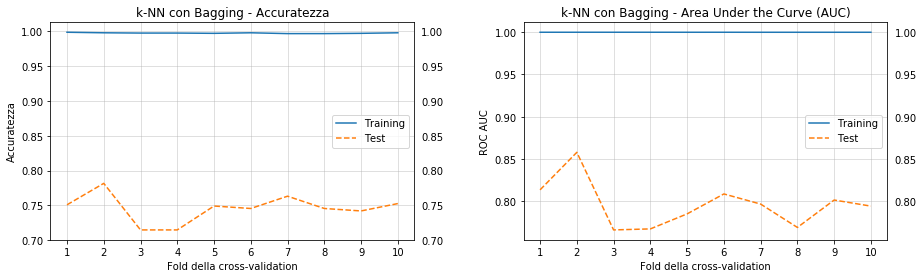
\includegraphics[width=\textwidth]{images/bagging.png}
	\caption{Risultati ottenuti applicando la tecnica di Bagging ad un classificatore k-Nearest Neighbor}	
	\label{fig:bagging}	
\end{figure}



\subsection{Classificazione con Boosting}
Come ultima tecnica di classificazione, si è scelto di applicare Boosting (in particolare usando l'algoritmo AdaBoost) alla SVM vincente della Tabella \ref{tab:svm}. 

Le prestazioni del modello aggregato sono state valutate mediante cross-validation, usando 10 fold. Il numero di classificatori istruiti e testati da AdaBoost per ciascuna fold è stato impostato a 20.

Sfortunatamente, i risultati ottenuti non sono stati quelli sperati: la Figura \ref{fig:boosting}, infatti, dimostra che le prestazioni del classificatore aggregato sono persino peggiori di quelle del modello singolo, senza contare l'alta variabilità (soprattutto nei valori della AUC) fra le varie fold.

\begin{figure}
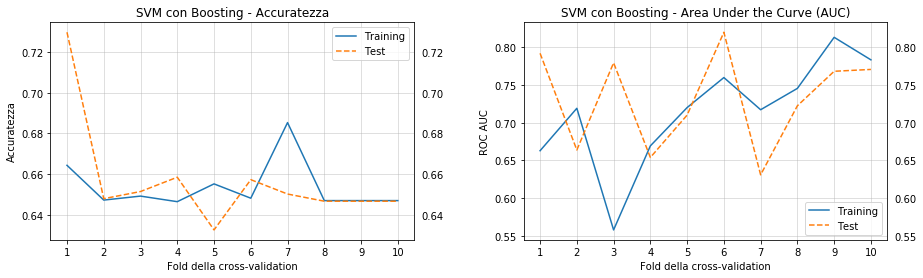
\includegraphics[width=\textwidth]{images/boosting.png}
\caption{Risultati ottenuti applicando la tecnica di Boosting ad una SVM}
\label{fig:boosting}
\end{figure}

\newpage

\section{Outlier Detection}

In questa sezione si illustra il processo di rilevamento degli \textit{outlier} sul dataset \textit{UCI Abalone} (lo stesso utilizzato nella precedente sezione). Lo scenario dei nostri esperimenti è quello \textit{Unsupervised}, cioè quello in cui non esistono elementi preventivamente etichettati come \textit{outlier}.

Nei successivi paragrafi saranno dunque impiegate tre diverse tecniche di rilevamento degli \textit{outlier} (appartenenti a diverse tipologie), allo scopo di confrontare i risultati ottenuti. In ognuna delle tre alternative, l'obiettivo è quello di rilevare l'1\% dei record del dataset che ha la maggiore probabilità di essere un \textit{outlier}. 

Per visualizzare i risultati in tre dimensioni, abbiamo utilizzato la \textit{Principal Component Analysis} (PCA), una tecnica di riduzione delle dimensionalità che tiene conto delle possibili correlazioni tra le varibili per operare una selezione delle \textit{feature} (\textit{Feature Selection}).

\subsection{Outlier detection tramite Local Outlier Factor (LOF)}

\textit{Local Outlier Factor (LOF)} è una tecnica di rilevamento degli \textit{outlier} appartenente alle varianti density-based. L'idea di base è comparare la densità relativa di un punto con quella dei suoi vicini: più essa si discosta dalle altre, maggiore è la probabilità che il punto sia un \textit{outlier}.

Nella Figura \ref{fig:lofs} sono mostrati i risultati ottenuti per tre diverse configurazioni del parametro \textit{n\_neighbors}, che definisce la quantità dei vicini  con i quali comparare la densità.

\begin{figure}[h]
\centering
\begin{subfigure}[b]{.32\linewidth}
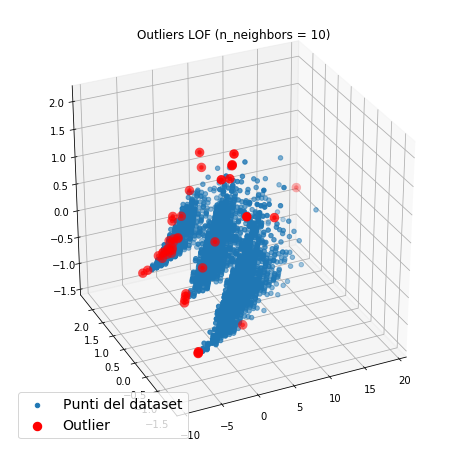
\includegraphics[width=\linewidth]{images/LOF_10.png}
\caption{n\_neighbors = 10}
\label{subfig:lof1}
\end{subfigure}
\begin{subfigure}[b]{.32\linewidth}
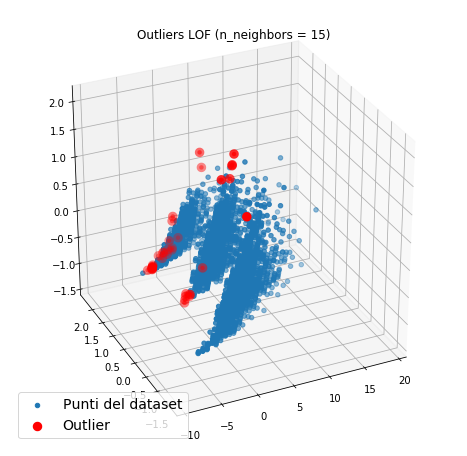
\includegraphics[width=\linewidth]{images/LOF_15.png}
\caption{n\_neighbors = 15}
\label{subfig:lof2}
\end{subfigure}
\begin{subfigure}[b]{.32\linewidth}
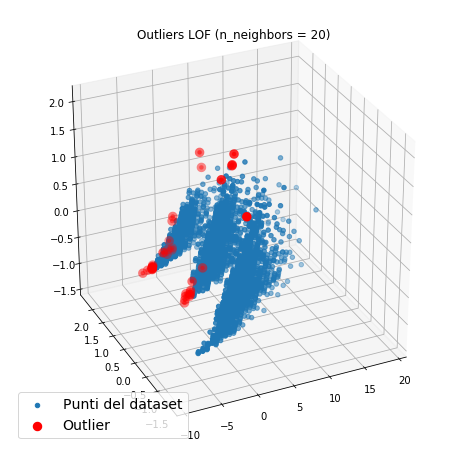
\includegraphics[width=\linewidth]{images/LOF_20.png}
\caption{n\_neighbors = 20}
\label{subfig:lof3}
\end{subfigure}
\caption{Outlier detection con Local Outlier Factor, per diversi valori del parametro \textit{n\_neighbors}}
\label{fig:lofs}
\end{figure}

\noindent
Ciò che salta immediatamente all'occhio è il fatto che, in ognuno dei tre casi, l'area di bassa densità situata nella parte in alto a destra del grafico non contiene quasi nessun \textit{outlier}. Infatti, nonostante la densità dei punti in quella regione sia piuttosto bassa, essa è relativamente omogenea. Piuttosto che classificarli tutti degli \textit{outlier}, LOF tende a considerarli come appartenenti ad uno stesso cluster a bassa densità.

Le aree nelle quali invece la presenza di \textit{outlier} risulta abbondante sono quelle che si trovano in prossimità  delle tre macro regioni ad altissima densità. La densità dei punti vicini a questi cluster, infatti, si discosta notevolmente da quella degli altri membri del \textit{reference set}, definito dal parametro \textit{n\_neighbors}. All'aumentare di quest'ultimo, osserviamo che continuano ad essere classificati come \textit{outlier} soltanto i punti la cui densità relativa è molto diversa da quelle degli altri punti nel rispettivo \textit{reference set} (Figura \ref{subfig:lof3}).



\subsection{Outlier detection tramite DB($\epsilon,\pi$) (DBSCAN)}

L'algoritmo di rilevamento degli \textit{outlier} DB($\epsilon,\pi$) fa parte degli approcci distance-based. In questo contesto, un punto viene considerato un \textit{outlier} se la percentuale di punti nel suo $\epsilon$-vicinato è minore o uguale a $\pi$. Intuitivamente, DB($\epsilon,\pi$) assume che i punti "normali" si trovino esclusivamente nelle aree ad alta densità. Nel seguito, il parametro $\pi$ è sostituito dall'equivalente $min\_pts$: invece di ragionare in termini di percentuale minima, ci riferiamo al minimo numero di punti che devono essere presenti nell'$\epsilon$-vicinato.

A differenza di LOF, questo metodo è particolarmente incline a localizzare gli \textit{outlier} in zone a bassa densità: piuttosto che su quella relativa, infatti, DB($\epsilon,\pi$) si basa su quella assoluta. Nella Figura \ref{fig:dbscans} sono riportati i risultati dell'algoritmo DBSCAN, per diversi valori dei parametri $\epsilon$ e $min\_pts$.

\begin{figure}[h]
\centering
\begin{subfigure}[b]{.32\linewidth}
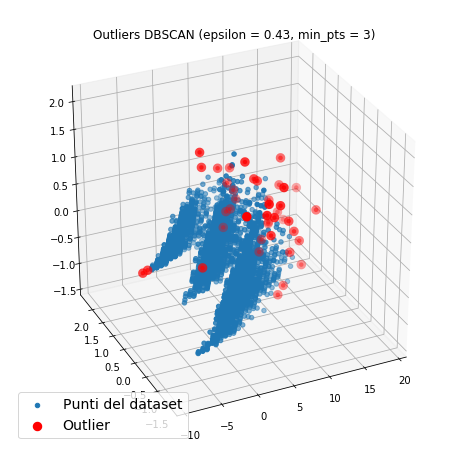
\includegraphics[width=\linewidth]{images/dbscan_min_pts_3.png}
\caption{min\_pts = 3, $\epsilon$ = 0.43}
\label{subfig:dbscan1}
\end{subfigure}
\begin{subfigure}[b]{.32\linewidth}
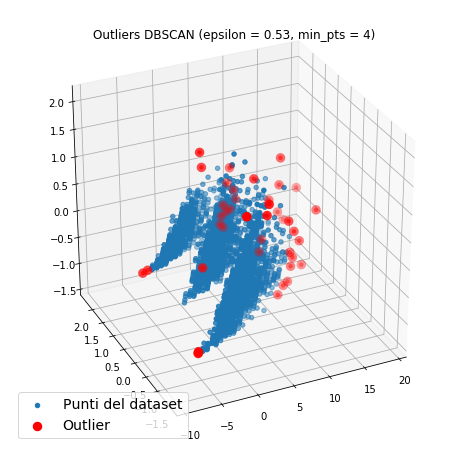
\includegraphics[width=\linewidth]{images/dbscan_min_pts_4.png}
\caption{min\_pts = 4, $\epsilon$ = 0.53}
\label{subfig:dbscan2}
\end{subfigure}
\begin{subfigure}[b]{.32\linewidth}
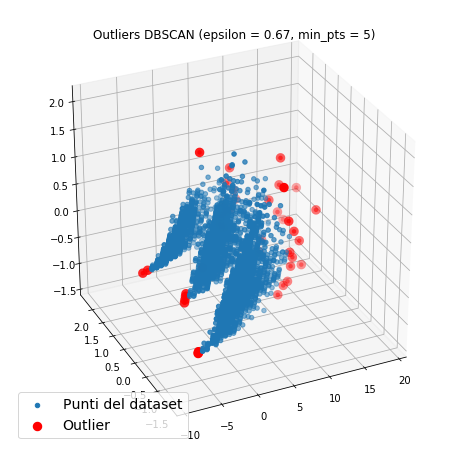
\includegraphics[width=\linewidth]{images/dbscan_min_pts_5.png}
\caption{min\_pts = 5, $\epsilon$ = 0.67}
\label{subfig:dbscan3}
\end{subfigure}
\caption{Outlier detection con DBSCAN, per diversi valori dei parametri \textit{min\_pts} e $\epsilon$}
\label{fig:dbscans}
\end{figure}

\noindent
In ognuna delle configurazioni, il parametro $\epsilon$ dipende da $min\_pts$ ed è stato scelto in modo tale che la quantità di \textit{outlier} rilevata costituisse l'1\% dell'intero dataset.

La differenza rispetto a LOF è sottolineata in maniera evidente dalla Figura \ref{fig:dbscans}: questa volta gli \textit{outlier} si concentrano proprio nell'area a bassa densità localizzata nella parte in alto a destra del grafico. Soltanto nella configurazione illustrata in Figura \ref{subfig:dbscan3} la situazione cambia leggermente: in tal caso, infatti, anche alcuni dei punti nelle estremità opposte dei tre cluster (intuitivamente, nelle loro "code") sono classificati come \textit{outlier}.

\subsection{Outlier detection con approccio depth-based}

L'ultimo degli approcci che abbiamo sperimentato è quello depth-based. Questa tecnica consiste nell'organizzare i dati in diversi livelli di inviluppi convessi (\textit{Convex Hulls}): l'assunzione principale è che gli \textit{outlier} si trovino nei livelli più esterni del dataset. La Figura \ref{fig:depth_based} mostra i risultati ottenuti.

\begin{figure}[h]
\begin{center}

	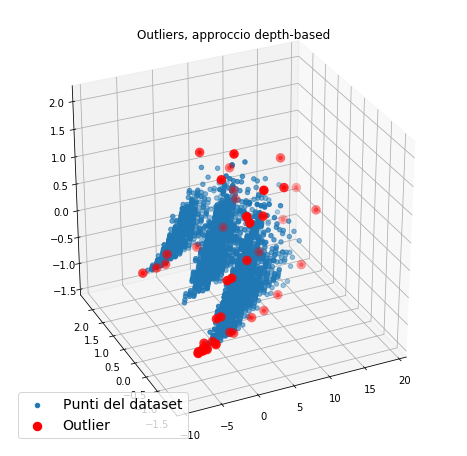
\includegraphics[width=.32\textwidth]{images/depth_outliers.png}
\caption{Outlier detection con approccio depth-based}
\label{fig:depth_based}
\end{center}
\end{figure}

\noindent
Rispetto alle due precedenti tecniche, si nota che gli \textit{outlier} si trovano sia in regioni a bassa densità (area in alto a destra del grafico) sia in prossimità di regioni ad altà densità (estremità inferiori dei cluster).
Questo tipo di approcci, infatti, non fa nessuna distinzione tra le densità relative e assolute dei punti. 

Sebbene l'idea di cercare gli \textit{outlier} ai confini del dataset possa sembrare sensata, a volte può rivelarsi un ostacolo. Tutti i punti situati nella parte centrale del dataset, per quanto possano essere isolati dagli altri, non saranno mai considerati \textit{outlier}. Una situazione del genere è illustrata nella Figura \ref{fig:depth_counterexample}.

\begin{figure}[h]
\begin{center}

	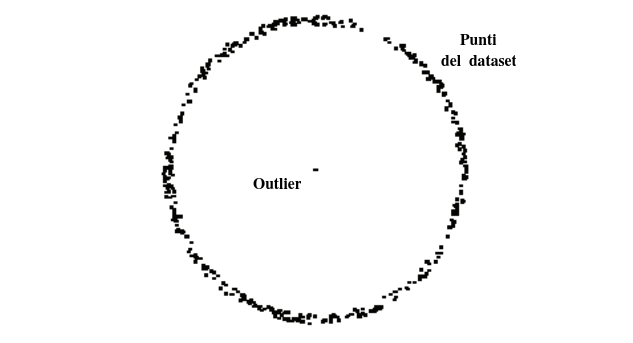
\includegraphics[width=.62\textwidth]{images/depth_example.png}
\caption{Scenario in cui gli approcci depth-based falliscono}
\label{fig:depth_counterexample}
\end{center}
\end{figure}

\subsection{Conclusioni}

In questa sezione abbiamo confrontato diverse tecniche di rilevamento degli \textit{outlier}, ognuna appartenente ad una diversa categoria (density-based, distance-based e depth-based). In particolare, abbiamo potuto constatare la profonda differenza tra i concetti di densità espressi da LOF e DB($\epsilon,\pi$): da una parte si considera la densità relativa ad un'area ristretta dello spazio (e quindi è ammessa la presenza di cluster di bassa densità), mentre dall'altra ci si riferisce alla densità relativa all'intero dataset. 

Gli esperimenti hanno infine dimostrato che, a seconda della distribuzione dei dati, possiamo ottenere sia ottimi che scarsi risultati: è opportuno dunque selezionare la tecnica ideale che più si addice alla situazione che abbiamo di fronte.

\bibliography{biblio} 
\bibliographystyle{apalike}

\end{document}
